\documentclass[a4paper,11pt,report]{article}
\usepackage[pdftex]{graphicx}
\usepackage{mathtools}
\usepackage[margin=0.9in]{geometry}
\usepackage{float}
\usepackage{lscape}
\usepackage{pdfpages}
\usepackage{epsfig}
\usepackage{epstopdf}
\DeclareGraphicsExtensions{.pdf,.png,.jpg,.eps}
\setlength{\parindent}{0in}

\begin{document}
\title{RentIt}
\author{Andreas Precht Poulsen, Morten F. Therkildsen, Mark Thorhauge, Toke Loke \& Mikkel Funch}
\date{28-05-2013}
\maketitle

\section{Introduction}
\subsection{Vision}
RentIt is a radio hosting service, that enables users to host online radio stations and for other users to listen to them.
It is a system intended to be used by the common user, without any special knowledge or traning.
\subsection{Glossary}
Track: An audio file that the users can listen to via channels. \\*
Channel: A collection of tracks that is played infinitly, and can be listened to by users. Managed by a channel host.

\section{Specification}
This section contains the functional and non-functional requirements, as well as the use cases that they are based on.
\subsection{Use Cases}
\textbf{Create account:}
The user navigates to the "create account"/"register" page. He fills out required information and agrees on possible conditions.

\textbf{Delete account:}
The user does not want to use the service any longer. He navigates to edit account and selects delete account. All data about the user is deleted accordingly.

\textbf{Listen to channel:}
The user navigates to the channel, possibly by searching for it and selects "listen to channel".

\textbf{Subscribe to channel:}
The user has selected a channel and selects "subscribe to channel". The subscription status changes accordingly.

\textbf{Unsubscribe to channel:}
The user has selected a channel he is already subscribed to and selects unsubscribe to channel. The subscription status changes accordingly.

\textbf{Comment channel:}
The user is on a channel and want to comment on it. He writes and submits the comment. The comment is saved and the page is refreshed

\textbf{Create channel:}
The user navigates to "create channel" and fills out the required information as well as uploading tracks. When the user is done it is immediately accessible by other users.

\textbf{Delete channel:}
The creater of the channel does not want the channel anymore and he decides to delete it. He navigates to edit channel and selects delete channel. All subscriptions to the channel are deleted, subscribers get notified, and the channel is removed.

\textbf{Upload track:}
The user has a channel and wants to upload a song. He navigates to edit channel. He selects the song through a filebrowser and selects upload.

\textbf{Delete track:}
The owner of a channel wants to remove a track from his channel. He navigates to edit channel. He browses the list of tracks and selects remove on the track he wants to remove.

\textbf{Edit channel:}
The owner of the channel selects edit channel and edits the channel attributes he wants to change. Then he confirmes the changes.

\textbf{Upvote/downvote track:}
The listener of a channel selects up- or downvote on a list of the last tracks that has been played.

\subsection{Functional requirements}
The functional requirements describe the required functionality of the system and defines enumerations for reference.
\\ \\
\textbf{R0:}
The system shall allow all users to create a channel, add attributes and edit it. \\*
\textbf{Domain concepts:}
The channel shall have its own collection of tracks that it plays and it is created and maintained by the channel host(the creator of the channel).
The channel shall have genres, a description and comments posted by users.
The channel must be visible to other users with prober search parameters. \\*
\textbf{Dependencies:} 
The requirement is nessecary for upload track and listen to channel because a track is associated with a channel. \\*
\textbf{Priority:} 
It is of essential importance, as the requirements depending on it is.
\\ \\

\textbf{R1:}
The system must allow users to listen to online radio-channel that streams audio. \\*
\textbf{Domain concepts:}
A channel has a collection of tracks that can be listened to. \\*
\textbf{Priority:}
Highest as this is the primary service that the system provides. \\*
\textbf{Implementation notes:}
The system must be able to stream audio in a smooth and clutter-free manner. The system must have an intelligent way of selecting the next track to be played, meaning that it must consider up/downvotes and how much it has been played.
A radio-channel must be able to stream an endless stream of audio without pauses between audio tracks.
Iit must be easy to write new clients for the service.
The interface for listening to audio must be as user friendly as possible.
\\ \\

\textbf{R2:}
The user must be able to rate a track associated with a channel. \\*
\textbf{Domain concepts:}
The rating of a track must affect the frequency with which it is played within its associated channel.
A higher rating giving a proportionally higher chance of being played. \\*
\textbf{Dependencies:}
The listen to channel requirement are depended on this requirement because the track to be played is determined by the rating.\\*
\textbf{Priority:}
It is of essential importance, as the requirements depending on it is.
\\ \\

\textbf{R3:}
It should be possible for users with a channel to upload a track to it. \\*
\textbf{Domain concepts:}
A channel has tracks that the creator manages. \\*
\textbf{Dependencies:}
The listen to channel requirement are depended on this requirement because the track to be played is determined by the rating.\\*
\textbf{Priority:}
It is of essential importance, as the requirements depending on it is.
 \\ \\

\subsection{Non-functional requirements}
The non-functional requirements describes how the functionality shall work in multiple aspects, as well as defining success criteria for them. They are structured with FURPS+. \\

\textbf{Functionality} \\*
\textit{Channels} \\*
Channel owners must be able to assign genre tags to the channels they control/own. \\*
Two users listening to the same channel at the same time must hear the same song with same amount of elapsed time (+- 1s), in other words, a channel is "playing" the same for all listeners. \\*
A function for searching for channels must be implemented. \\*
A list of the most popular channels should be available to all users. Popularity must be based on an algorithm and it must be explained in the documentation. \\*

\textit{Tracks} \\*
The service must support tracks in .mp3 format. \\*

\textit{Logging and Error Handling} \\*
All exceptional states must be logged.\\*
All state changes must be logged.\\*

\textit{Security} \\*
All usage requires authentication. (usage meaning the use of any services related to the program)\\*

\textbf{Usability} \\*
The website should be intuitive to use for 90\% of persons above the age of 12 with regard to the following:
\begin{itemize}
\item listening to a channel
\item maintaining one 
\item uploading songs
\item voting
\item subscribing
\end{itemize}

There must be help available for all functions in the form of text. This help must be accessible from within the client \\*
Users must not be required to subscribe to a channel in order to listen to it. \\*
Users must be required to be subscribed to a channel in order to vote on the channel. \\*
If a user unsubscribes from a channel, all votes made by that user must be removed so as to not affect track ordering. \\*
Users must be able to see all the songs contained in a channel. \\*
Users must be able to upvote and downvote the last 5 songs that have been played on the channel while they were listening. \\*
Users must not be required to download or install any third party software in order to listen to a channel. \\*

\textbf{Reliability} \\*
The server must not be affected by any errors clientside. All operations requires internet connection. No system failure of any kind should affect any track in the persistence storage. \\*
If a channel on the server crashes:
\begin{itemize}
\item all clients must be notified about the failure.
\item the website must not be affected by the crash.
\item the website must refresh the website with possiblity to listen to the channel greyed out until the channel have been fully recovered on the server side.
\item on the server side, the channel stream must shut down.
\item the error must be logged and reported automatically. 
\item the channel must be safe to use again when all track's identity have been confirmed(via hashing), and none of them are in use.
\end{itemize}
If upload of a track fails, everything about the track must be removed from the server and the user must be notified. \\*

\textbf{Supportability} \\*
The server architecture may not limit the ability to correct eventual errors. This means that no unessesary coupling exists in the server.
The server and website must be implemented modular so as to ease extendibility.
This means that extensions such as video streaming or downloading of media must not requrie extensive changes in the system architecture. \\*
The server will be running on Windows Server 2008 R2 Enterprise OS with support of .NET 4.0 Framework.\\*

\textbf{Implementaion} \\*
The server will be written in C\# with the .NET 4.0 Framework and Windows Communication Foundtaion.
The website will be written in ASP.NET and must work in all popular browsers.

\subsection{Target Audience}
The target audience of our RentIt Radio system is primarily users in the age 13-35. Since our system is not just a place to listen to music, but also a place to discuss music,  older users might choose ordinary radiostations. Younger people are more used to social networks and the radio system is designed to be a social network combined with radio.

\section{Analysis}
This section contains considerations on how to implement the functional and non-functional requirements. This includes the possible solutions, the chosen solution and the reasoning for the choice.

\subsection{Datamodel}
The basic domain entities of the system consists of channel, user and track. The rest of the entities supports functionality that is required for the basic entities. \\*
User and channel each represents a unique system entity, while track can represent the exact same data as another track, only seperated by the id and the channel it belongs to.
The decision to not let channels share tracks is because it would require analysis of the mp3 file, to determine whether it is similar, regardless of the name/artist combination.
This design does not limit a possible extention of the system to measure similar mp3 files and update references to avoid redundant data in the file system.
Such an extension does not remove redundant data in the database, which our datamodel does not support. Track has a upvote and downvote count, which vote entities have a functional dependency to,
because for each vote on a track, upvote or downvote is increased. This duplication is made to speed the algorithm, because it does not need to count vote entities when it has counts. \\*
The vote entity exists to prevent users from voting one track several times.
TrackPlay is an entity that represents a play of a track. It is an entity and not an attribute of track, because we want to record the date it was played. \\*
Genre is an entity and not an attribute of channel because we want to make a fixed set of genres to choose from when creating a channel.

\subsection{Data storage}
For storing information about our data classes. Microsoft SQL Server has been chosen because it is integrated with the server. The reason for choosing a DMBS\footnote[1]{Abbreviation for Database Management System} to store most of our data in is because it is fast and optimized for storing and retrieving data. However a research paper[reference] suggests that when it comes to object with size beyond 1MB it is faster to store the object on the file system. Due to the knowledge acquired from the paper we chose to store our music files on the file system, because the average size of an mp3 file is around 3-4MB. We have a table called track which have a path that indicates where the song is placed on the file system.

\subsection{Webservice}
The return types of most methods is straightforward. Methods which have at most one result will return the corresponding object, wrapper object in case it is an object which should reflect an object in the database, such as a channel or a user. \\
With methods which typically have more than one result, we have more options(methods like GetTrackIds and GetChannelIds). 
The first option is to return an array of the ids of the result. The second option is to return an array with all the objects that corresponds to those ids. And the third option would be to return lazy objects, which were first completed(retrieved from the server) when the client called methods upon them. By returning an array of ids we allow the client to decide which objects they actually want to use time and bandwidth retrieving completely. By returning all objects we force the instantiation of all objects in the server. And by using lazy objects we allow low bandwidth and only a single network transfer at first and wait till the objects are actually needed.
The returning of ids give the clear advantage of giving complete control to the client. When the client retrieves an array of ids, it can decide for itself which objects it actually needs. The disadvantage for this is that our webservice api needs methods for retrieving single objects from id and the client have to call this method for each object it needs. \\
The advantage for sending all objects back in the first method call is that there will only be one method call and only one network-transfer. The disadvantages is that this could get really rough on the bandwidth and server load as some objects might contain images and other types of heavy properties and all objects would have to be completely instantiated. Another thing is that the client would have to handle this, possibly, huge load of objects even though it might not need to use most of them. \\
The advantage of lazy object instatiation is that it potentially loads fewer objects. The actual object instantiation and retrieval is done when it is needed the first time. A massive problem with this is, that the load times would be unstable even when the site is completely loaded. Simple clicks or hovers, which requires some new information, would have to make a new network transfer. \\
We have chosen to implement the solution which returns ids. This allows for several network transfers but the possibility of making the workload on the bandwidth and the server as low as possible for what is actually required. The problem with lazy objects is that people want a fully loaded website to actually be completely loaded and not have to wait for some objects, which is shown to be there, but isn't actually loaded. \\
In the method GetChannelIds (the method used for searching in all channels) we have chosen the input to be an instance of SearchArgs. The SearchArgs class cointains properties for all the different arguments we allow to search on, this way we have one method which takes one argument, rather than a method which takes parameters for every single property we have in SearchArgs. \\
All objects we return, which is a representation of data from our database, will be returned as a customized wrapper object. This is in order for us to be in complete control of what we return to our clients and in order to keep our internal structure as hidden as possible. If we returned raw objects created by our entity framework, we would expose data which is not relevant for the user and could be used to hurt the server, for example filesystem paths.

\section{Implementation}
This section describes how the system is implemented by describing classes with a class diagram and dynamics with sequence diagrams.

\subsection{Major classes}
\textbf{Dao} \\*
Communication with the database is done through a single data access object. This object functions as a bridge between the database and the server program, and it enables basic CRUD operations on the database for the server program. 

\textbf{FileSystemHandler} \\*
Communication with the filesystem on the server is done through a single data access object. This object functions as a bridge between the filesystem and the program on the server. It enables the same basic operations on the filesystem as the Dao does on the database

\textbf{RentItService} \\*
All communication between clients and the server go through this webservice class. It supports all the operations necessary to fulfill the requirements for the program. 

\textbf{TrackPrioritizer} \\*
This class manages the prioritizing of tracks being returned to the client, fulfilling the requirements about the order of tracks being played.

\textbf{Controller} \\*
This class is the single point of entry to the server programs functionality.

\newpage
\subsection{Class diagram}
\begin{figure}[H]
  \centering
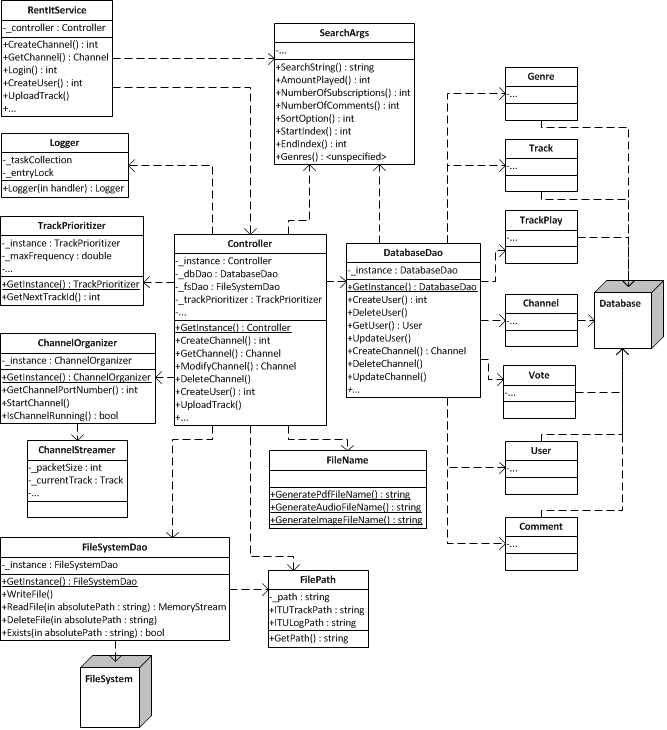
\includegraphics[]{./ClassDiagram.png}
\caption{Class diagram of important methods and all classes}
\end{figure}

\begin{landscape}
\subsection{Sequence diagram}
\begin{figure}[H]
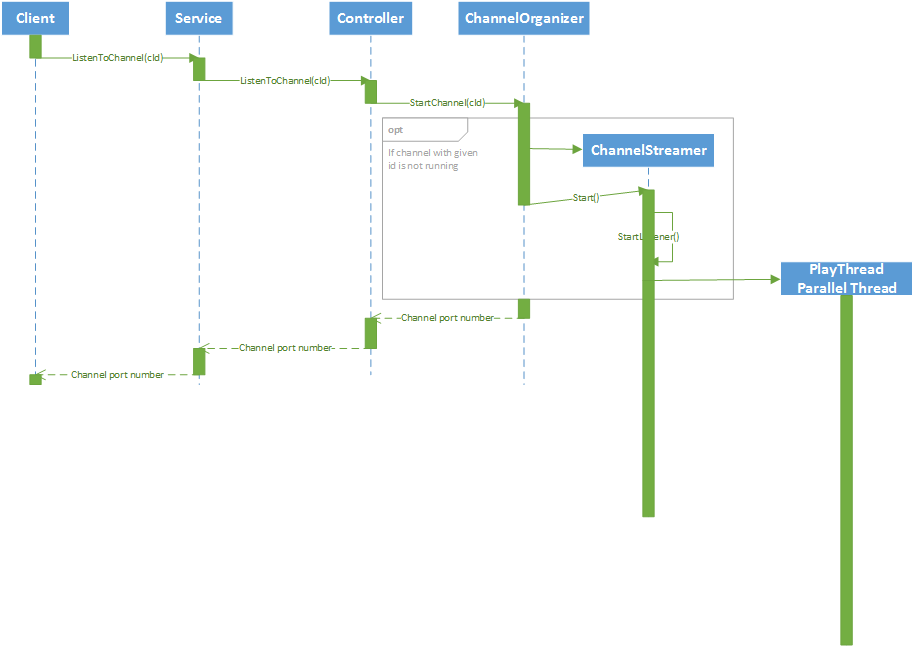
\includegraphics[]{./ListenToChannelSD.png}
\end{figure}
\end{landscape}


\section{Collaboration with SMU}

\subsection{Interaction with the ITU system}
As both the ITU system and the SMU system is an IS\footnote[2]{Abbreviation for Information System} and deployed on the same server,  some of the classes have been reused in the SMU system and the ORM\footnote[3]{Abbreviation for Object Relation Mapping} is in the same entity framework.
The classes that have been reused are in the utilities namespace, and are FilePath, FileSystemHandler and Logger. We have designed the classes in such a way, that a method call in one system can't affect the other system. \\
The success criteria for our systems is that an error or change in one system should not affect the other if not intended. Two different web services have been used to avoid that an erroneous method affects the other system.
The drawback to this decision is that the clients cannot share web service methods without adding the other web service. However, none of the client needs the web service of the other system. 

\subsection{SMU webservice api}

The following api is the api the group from Singapore requested. 

\begin{itemize}
	\item int SignUp(string email, string name, string password, bool isAdmin)
	\item int LogIn(string email, string password)
	\item User GetUserInfo(int userId)
	\item User UpdateUserInfo(int userId, string email, string username, string password, bool? isAdmin)
	\item void DeleteAccount(int userId)
	\item Book[] GetAllBooks()
	\item Book[] GetPopularBooks()
	\item Book[] GetNewBooks()
	\item Book[] SearchBooks(String searchString)
	\item Book[] GetBooksByGenre(String genre)
	\item Book GetBookInfo(int bookId)
	\item int HasRental(int userId, int bookId)
	\item Rental[] GetRental(int userId, int bookId)
	\item int RentBook(int userId, int bookId, int mediaType)
	\item MemoryStream DownloadPdf(int bookId)
	\item MemoryStream DownloadAudio(int bookId)
	\item MemoryStream DownloadImage(int bookId)
	\item Rental[] GetActiveUserRentals(int userId)
	\item Rental[] GetAllUserRentals(int userId)
	\item void DeleteBook(int bookId)
	\item int UploadBook(string title, string author, string description, string genre, double price, MemoryStream image)
	\item Book UpdateBook(int bookId, string title, string author, string description, string genre, double? price, MemoryStream image)
	\item void UploadAudio(int bookId, MemoryStream mp3, string narrator)
	\item void UploadPdf(int bookId, MemoryStream pdf)
\end{itemize}












\end{document}